% IEEE standard conference template; to be used with:
%   spconf.sty  - LaTeX style file, and
%   IEEEbib.bst - IEEE bibliography style file.
% --------------------------------------------------------------------------

\documentclass[letterpaper]{article}
\usepackage{spconf,amsmath,amssymb,graphicx}

% Example definitions.
% --------------------
% nice symbols for real and complex numbers
\newcommand{\R}[0]{\mathbb{R}}
\newcommand{\C}[0]{\mathbb{C}}

% bold paragraph titles
\newcommand{\mypar}[1]{{\bf #1.}}

% Title.
% ------
\title{Optimizations on the Pentagon Abstract Domain}
%
% Single address.
% ---------------
\twoauthors{Erik Henriksson}{ETH Z\"urich\\Z\"urich, Switzerland}{Boris Peltekov}{ETH Z\"urich\\Z\"urich, Switzerland}

\usepackage{color}
\newcommand{\erik}[1]{\textcolor{blue}{[Erik: #1]}}

% For example:
% ------------
%\address{School\\
%		 Department\\
%		 Address}
%
% Two addresses (uncomment and modify for two-address case).
% ----------------------------------------------------------
%\twoauthors
%  {A. Author-one, B. Author-two\sthanks{Thanks to XYZ agency for funding.}}
%		 {School A-B\\
%		 Department A-B\\
%		 Address A-B}
%  {C. Author-three, D. Author-four\sthanks{The fourth author performed the work
%		 while at ...}}
%		 {School C-D\\
%		 Department C-D\\
%		 Address C-D}
%

\begin{document}
%\ninept
%
\maketitle
%

%The hard page limit is 6 pages in this style. Do not reduce font size
%or use other tricks to squeeze. This pdf is formatted in the American letter format, so may look a bit strange when printed out.

\begin{abstract}
%Describe in concise words what you do, why you do it (not necessarily
%in this order), and the main result.  The abstract has to be
%self-contained and readable for a person in the general area. You
%should write the abstract last.
In this work we present an implementation of join on the Pentagon Abstract Domain. We explain the basics of the operation, the improvements which is possible of the naive implementation and conclude with our resulting SIMD vectorized version. Our work gives insight in the huge benefits one can get by optimizing data storage and utilizing the vector instructions which are available on modern Intel processors. We hope this work will be useful to improve the performance on future program analyzers.
\end{abstract}

\section{Introduction}\label{sec:intro}
Many huge bugs in computer science history has been caused by accessing array out-of-bounds, especially in the form of buffer overflow errors. %http://crypto.stanford.edu/cs155/papers/cowan-vulnerability.pdf
The domain of abstract intrepretation has therefore gotten attention from researchers and new domains as the octagon and polyhedra domain has been invented. These allows to also capture relations between variables, something which is very useful when you want to prove invariants about array accesses. The ``classical'' interval domain is an example of a domain which is not precise enough to prove this. The main property you have to sacrifice for preciseness is speed.

\erik{TODO: Add Intel's manual to the list of citations}

\erik{Replace subsections with mypars if you need extra space}

\mypar{Motivation} Logonzzo et al. proposes a new domain, Pentagon Abstract Domain, which allows for capturing intervals and strict upper bounds between variables. We have looked into this domain to optimize the most critical operations on the Intel Core architecture. We have found the join operation or more specifically the transitive closure performed inside a join to be the most critical and has thus focused our work on that operation.

\mypar{Related work} There is a paper from P\"uschel et al. which explains how to do tiling and vectorization of the Floyd-Warshall algorithm, which also we use in the transitive closure. However, since this work is done on general graphs and our work is done on the special case where all edges have equal length, there is considerable amount of optimization. There is also an excellent manual from Intel, Intel® 64 and IA-32 Architectures Optimization Reference Manual, which has proven very useful for us. 
%Do not start the introduction with the abstract or a slightly modified
%version. It follows a possible structure of the introduction. 
%Note that the structure can be modified, but the
%content should be the same. Introduction and abstract should fill at most the first page, better less.

%\mypar{Motivation} The first task is to motivate what you do.  You can
%start general and zoom in one the specific problem you consider.  In
%the process you should have explained to the reader: what you are doing,
%why you are doing, why it is important (order is usually reversed).
%
%For example, if my result is the fastest DFT implementation ever, one
%could roughly go as follows. First explain why the DFT is important
%(used everywhere with a few examples) and why performance matters (large datasets,
%realtime). Then explain that fast implementations are very hard and
%expensive to get (memory hierarchy, vector, parallel). 
%
%Now you state what you do in this paper. In our example: 
%presenting a DFT implementation that is
%faster for some sizes than all the other ones.
%
%\mypar{Related work} Next, you have to give a brief overview of
%related work. For a paper like this, anywhere between 2 and 8
%references. Briefly explain what they do. In the end contrast to what
%you do to make now precisely clear what your contribution is.

\section{Background: Abstract interpretation and Transitive closure}\label{sec:background}

In the field of Abstract Interpretation the ``join'' operation between two abstract 
domains is one of the most commonly used, because it is responsible for correctly 
merging the inferred information coming from two different program flow paths. 
Since most programs heavily rely on branching, the ``join'' operation must be perfected 
both in terms of speed and correctness -- it has to preserve as much information as possible, 
but also overapproximate the information coming from the merging paths. 
Note that there is an instantiation of the abstract domain at every program point 
and information is exchanged between them -- the join operation is one example of 
such exchange. More specifically, every Pentagon domain \cite{Logozzo2008} consists of two 
subdomains -- interval and strict upper bounds (SUB). The interval subdomain 
contains a mapping from a variable to an interval of possible values, which 
the variable may take. In case when no bounds can be inferred, the variable 
is mapped to an artificial interval called TOP. The SUB domain is a set of 
strict inequalities between variables with the requirement that all of them 
must hold at the given program point. Note that no inequalities between expressions are allowed.

\subsection{Mechanics of Pentagon join}
Before joining the two domains, a closure operation is performed on each one of them. 
Its purpose is to enrich (in terms of precision) and exchange the available 
information between the SUB and interval subdomains. The closure can be described in 3 steps:
\begin{enumerate}
\item Infer stricter interval bounds given some inequalities. 
For example if \(a \in [2,8]\), \(b \in [0,6]\) and \(a < b\) one could deduce that \(a \in [2,5]\) and \(b \in [3,6]\).
\item Infer inequalities given some intervals. 
For example if \(a \in [2,5]\) and \(b \in [8,10]\) then one could safely infer that \(a < b\).
\item Transitive closure of SUB domain. If \(a < b\) and \(b < c\) then \(a < c\).
\end{enumerate}
It must process the SUB domain until reaching a stable point. More applications of transitive closure would not change the data.
Once closure is applied to both domains, the join is delegated to interval and SUB domains respectively. 
They strictly adhere to the mantra of overapproximation -- the result should be sound in the 
sense that no possible data assignment is missed. In case of intervals -- if \(a \in [2,5]\) in 
the first domain and \(a \in [7,12]\) in the second, the join should be at least \([2,12]\). 
Of course, further inflation of the result would not affect the soundness, but 
the precision will suffer, therefore it is undesireable. 
The same applies to SUB join -- if an inequality is present in only one of the domains, it should not be included in the result.

\subsection{Cost analysis}
From now on we assume that the SUB domain is encoded as n by n matrix of 0's and 1's 
where n is the number of variables. 1 on ith row and jth column would designate 
that ith variable is less than jth variable. Steps 1 and 2 of the closure 
take \(O(n^2)\). Step 3 takes \(\Theta(n^3)\). It can be implemented using the Floyd-Warshall 
algorithm \cite{Floyd1962} augmented with logical operations – 1 AND and 1 OR in the innermost 
loop, thus the exact number of logical operations is \(2n^3\). We do not include in the cost measure
the operations needed for updating the loop indices. The interval join is 
linear and the SUB join takes \(O(n^2)\). In conclusion, the costliest step is 
the transitive closure of the SUB domain, therefore we concentrated our efforts 
to optimize it, taking the Floyd-Warshall algorithm as a starting point. 
Taking into account that in a single Pentagon join the transitive closure is 
performed twice, the total cost of a Pentagon join is \(4n^3 + O(n^2)\) operations.


\section{Optimized Transitive closure}\label{sec:yourmethod}


\subsection{Naive implementation - STL}
We started with implementation of transitive closure using STL library. 
It uses STL maps and sets to encode that variable x is less than every 
variable in a given set. It is very concise in terms of memory 
footprint -- it doesn't waste any space and supports runtime-varying 
number of variables, but a major downside is that the STL maps and sets 
use Red-Black trees, which generally do not exhibit any spacial locality. 
The STL implementation proved to be much slower than the others and there 
is no much to do about it, because, as the profiling investigation 
confirmed, most of the time is spent in STL internals.

\subsection{Better na\"ive implementation – Dense matrix (DM)}
For the DM implementation we switched to different representation of the 
SUB domain – n by n matrix of 1's and 0's. On top of it runs the standart 
Floyd-Warshall (FW) algorithm (with conditionals after the 2nd and 3rd loop). 
Because of these conditionals the op count may be less than \(2n^3\). The DM 
and STL implementation yielded the same results, thus we used them as a 
basis for our verification framework. For the sake of comparison, the DM 
proved to be much faster than the STL implementation, because the data is 
packed in only one array and there is no extra auxiliary information stored (not the case with STL primitives).

\subsection{Opportunities for improvement}
The first step is to replace the conditionals from FW with logical operations. 
This streamlines computation and paves the way for further optimizations 
(bit-packing and SIMD processing). The downside is that the op count now is exactly \(2n^3\). 
After this step the FW superficially resembles the matrix-matrix multiplication (MMM), 
for which there are widely known and efficient optimizations such as loop reordering, 
tiling for cache/registers, loop unrolling. After a closer look to FW, it's evident 
that the k loop should be the outermost one and i and j loops do not depend on each 
other -- therefore they can be reordered.

It is known that putting i as the outermost loop is superior in MMM, but this is 
not possible in our case, which explains why MMM-like performance is not achieveable. 
The algorithm with k,i,j loop order shows spacial locality, because for every k-step the matrix is traversed 
in row-major order which coincides with the memory layout of the array (in C).
Between successive iterations of k temporal locality is exhibited, but since k is the outermost loop and 
inside it the whole matrix is traversed, there is a benefit only when the whole matrix fits in last-level cache (n is small). Because of 
this fact, tiling for cache is crucial for achieving top performance in cases 
when n is large. Due to the independence of i and j loops, we introduced 
tiling on them (with configurable parameters) and observed tangible performance improvement.

\subsection{Tiling for cache}
The restriction on the k loop is imposed by data dependencies 
(otherwise the algorithm would not compute the full transitive closure), 
but as shown in \cite{Pueschel2006}, it can be relaxed through creating 
a FW version (FWabc) which works on 3 mutually distinct matrices (two “source” and one “destination”) 
rather than 1. In this special version the loops can be freely reordered 
and tiled. In order to unleash the potential of this optimization, tiling 
of the input matrix is needed. As next step of optimization process we 
implemented tiled version of FW (FWT, with configurable parameters) following 
the approach described in \cite{Pueschel2006}. The 
essence of it is to call FWabc whenever possible (when 3 distinct submatrices are encountered) 
during the processing of smaller submatrices. We observed about 4x improvement 
compared to na\"ive DM for large n (there is no big difference for small n, because 
the workset of DM fits in the cache). After that we started experimenting with 
different tile sizes -- the only restriction is that n should be divisible by the 
tile size. The workset of DM consists of the whole matrix, whereas the workset 
of FWT is 3 tiles. We experimented with various workset sizes and found that 
crossing the L1 cache threshold doesn't affect performance, but when the workset 
gets bigger than the L2 cache, the performance is severely degraded. Based on our 
benchmarks, we decided not to implement two levels of tiling, but rather 
concentrate on loop unrolling and fine-tuning the innermost basic block.

Now we examine the operational intensity of DM and FWT to see if they are memory bound.
We measure the memory traffic by approximating the number of cache misses. Let $c$ be the cache size, $s$ - cache block size (64 bytes in case of Core 2), 
$b$ - block size (in FWT) and $M=\frac{n}{b}$ is the number of tiles in one row.
From now on we assume that $n>>c$. In DM, if k and i are fixed, there will be $\frac{2n}{s}+1$ misses. In total there will be $\frac{2n^3}{s}+n^2$ misses.
The number of ops is $2n^3$, so the operational intensity is $I(n) = \frac{2n^3}{2n^3+sn^2} = \frac{2n}{2n+s} \in O(n)$.
In FWabc, if $c>3b^2$(i.e. the workset fits in cache), the operational intensity will be $\frac{2n^3}{3b^2}$, because the data will be loaded just once from memory.
Following the scheme of FWT in \cite{Pueschel2006}, we count the number of tiles that need to be loaded during the computation and use it to calculate the cache misses and
the operational intensity. If k is fixed, the first three phases load $2(M-1)+1$ tiles and phase 4 loads $(M-1)(2M-1)$ tiles. Loading of each tile costs $\frac{b^2}{s}$ cache
misses. In total there will be $(2M^3-M^2)\frac{b^2}{s}$ misses and after substitution of $M=\frac{n}{b}$ the result is $\frac{2n^3}{bs}-\frac{n^2}{s}$ misses. Note that the op count
in FWT is still $2n^3$. So if we choose $b=\sqrt{\frac{c}{3}}$, the amount of bytes transferred will be at most $\frac{2\sqrt{3}n^3}{\sqrt{c}}$ bytes. The gain is approximately 
$2\sqrt{c}$ and the operational intensity is $O(\sqrt{c})$. This explains the performance advantage of the tiled version and also confirms that it is not memory bound.

\subsection{Loop unrolling and scalar replacement}
During the development of all variants of Pentagon join, we used configurable 
compile-time unrolling parameters and compiler flags and pragmas to hint 
the compiler which loops to unroll. The motivation for this decision is 
the possibility to automatically find good values for the unrolling factors. 
After finishing the bit-packed and SIMD implementations, we searched for 
the ``sweet spots'' of unrolling parameters using scripts. Taking them as a 
reference point and considering the number of available registers and the architecture of the Intel Core 2 processor, 
we implemented hand-written single static assignment (SSA) basic blocks using 
scalar replacement to avoid pointer aliasing. In principle some of the code (namely FWabc) 
operates on distinct arrays, so we used this fact during the development of the basic blocks. 
We strived to utilize the ideas found in micro-MMM (register blocking and reordering 
for instruction level parallelism), but there is a lower degree of register reuse in Floyd-Warshall than in matrix-matrix multiplication.
% However both in FW and FWabc there is a low degree of register reuse and the results showed similar or even a bit lower performance when using the optimized basic blocks.

%\erik{TODO: Add bit-packing and SIMD -- Make sure to explain the details about SSE register expanding and loop order}
\subsection{Bitpacking}
An important step is to notice that we use boolean matrices and therefore can make use of bit-packing to reduce both memory footprint and increase the number of ops/cycle the processor can perform. The main idea is to represent every element by a bit instead of an integer. We also had to convert some of the binary operations to use the bit-wise variant. This is of course also possible in a SIMD implementation using the SIMD variants of the regular bit-wise operations.

\subsection{Theoretical performance analysis}
The objective of the theoretical analysis is to approximate the upper bound on performance of our SIMD implementation
achievable on a particular piece of hardware and to pin-point the bottlenecks. Now we will examine our 
SIMD implementation with all previously described optimizations applied. 
The loop order inside the tiles is k,i,j -- so no distinction between FW and FWabc is needed in this regard. 
There are three major places where a bottleneck can occur:
\begin{enumerate}
\item CPU's arithmetic resources - number of ALU's, distibution of the operations over the execution ports etc. 
\item CPU-cache bandwidth (and sometimes latency)
\item Cache-RAM bandwidth
\end{enumerate}

In order to update a single 128-bit chunk of data C[i,j:j+128] two logical SSE operations are needed -- 1 AND and 1 OR. Despite that the OR depends on the AND, 
high throughput can still be achieved, because these operations for different j and fixed k,i can be done in parallel. So given the unrolling on j and hardware capable of
out-of-order execution, this dependency would not be an issue. Our test hardware has 2 (Core 2 Duo) or 3 (Ivy Bridge) execution ports capable of processing a SSE logical operation 
each cycle. Considering only this, the peak performance should be 256 or 384 ops per cycle respectively. However there are other obstacles which prevent achieving this. 

Now lets focus on the memory behaviour of the algorithm. Inside the i loop one particular bit (A[i,k]) has to be extracted and its value spread along a SSE register. Then this value is 
used during the whole j loop. Therefore, assuming enough work done in the j loop, the effect of this memory load is negligible. 
Inside the j loop there are 2 SSE loads and 1 SSE store that need to be done. However the Sandy Bridge has only 1 load and 1 store port, so it is capable of
only 1 load and 1 store per cycle. Consequently this limits the performance to 128 ops per cycle. We tried to alternate the dataflow of the algorithm, but we could not
evade the stream-processing nature of the inside the j loop -- two 128-bit values are fetched, 2 SSE operations are applied and then the result is written back. 
Despite that the distinct iterations of j are completely independent both in terms of memory usage and arithmetic operations, the 
bottleneck is the L1 cache bandwidth. No further data or register reuse is possible given our implementation layout. The positive side of it is that the data is accessed 
linearly row-wise and would not cause any unnecessary cache misses.
% We also experimented with i,j,k loop layout inside a tile, but it exhibited ...

As discussed in section 3.4, the tiled FW is not memory bound and the slow RAM-cache bus will not impede its performance. As a result of the shown reasoning we conclude that no more than 
128 ops per cycle can be sustained on our test hardware. Not suprisingly, the results confirm that -- about 110 ops per cycle were achieved in our benchmarks. We attribute the performance gap to the fact that 
the execution ports for the logical SSE operations are shared with the ALUs responsible for incrementing the indices and calculating the memory addresses.

\section{Experimental Results}\label{sec:exp}
%\erik{Erik will write this ; Also include proper explanation of the results}
%\erik{Maybe it's a good idea to share a link to github or directly give it to Pueschel}
We ran all the tests on an Intel Core i7-3615QM, 2.3 GHz, Mac OS X 10.9 64-bit OS. We have written a benchmark suite which we used for our benchmarks. We used GCC 4.9 with \textsf{-O3} optimizations enabled.

We analyzed performance for different config values we use in the code to find the sweet-spot for this particular CPU. The benchmark suite is named \textsf{benchmark.cpp} and can be found in the repository. 

We have implemented four different variants of the algorithm; as described in the paper using STL maps, using dense matrix, using bit-packed matrix and using SIMD bit-packed matrix. 

\begin{figure*}
  \centering
  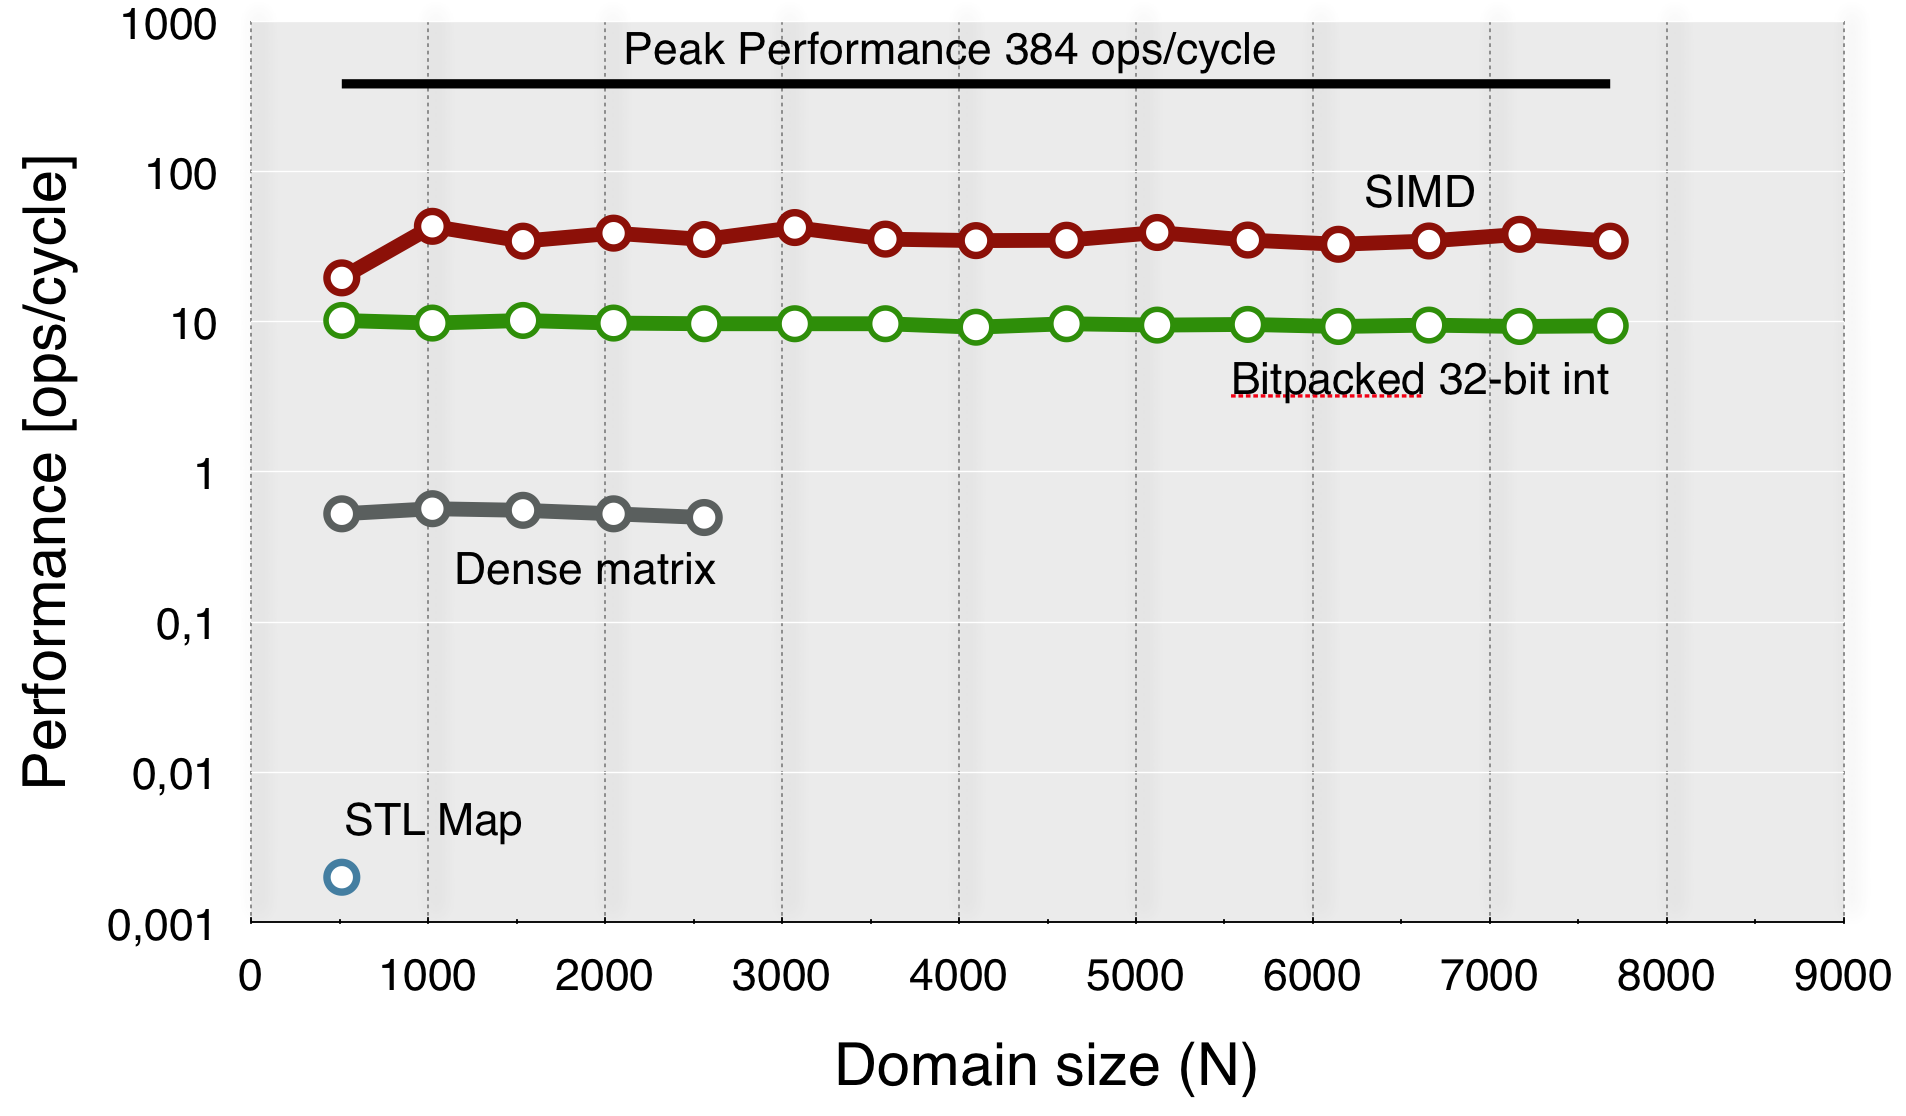
\includegraphics[width=0.85\textwidth]{graphs/Domain_size.png}
  \label{fig:benchmarking-results}
  \caption{Comparison of the four different implementations for different domain sizes}
\end{figure*}

\begin{figure*}
  \centering
  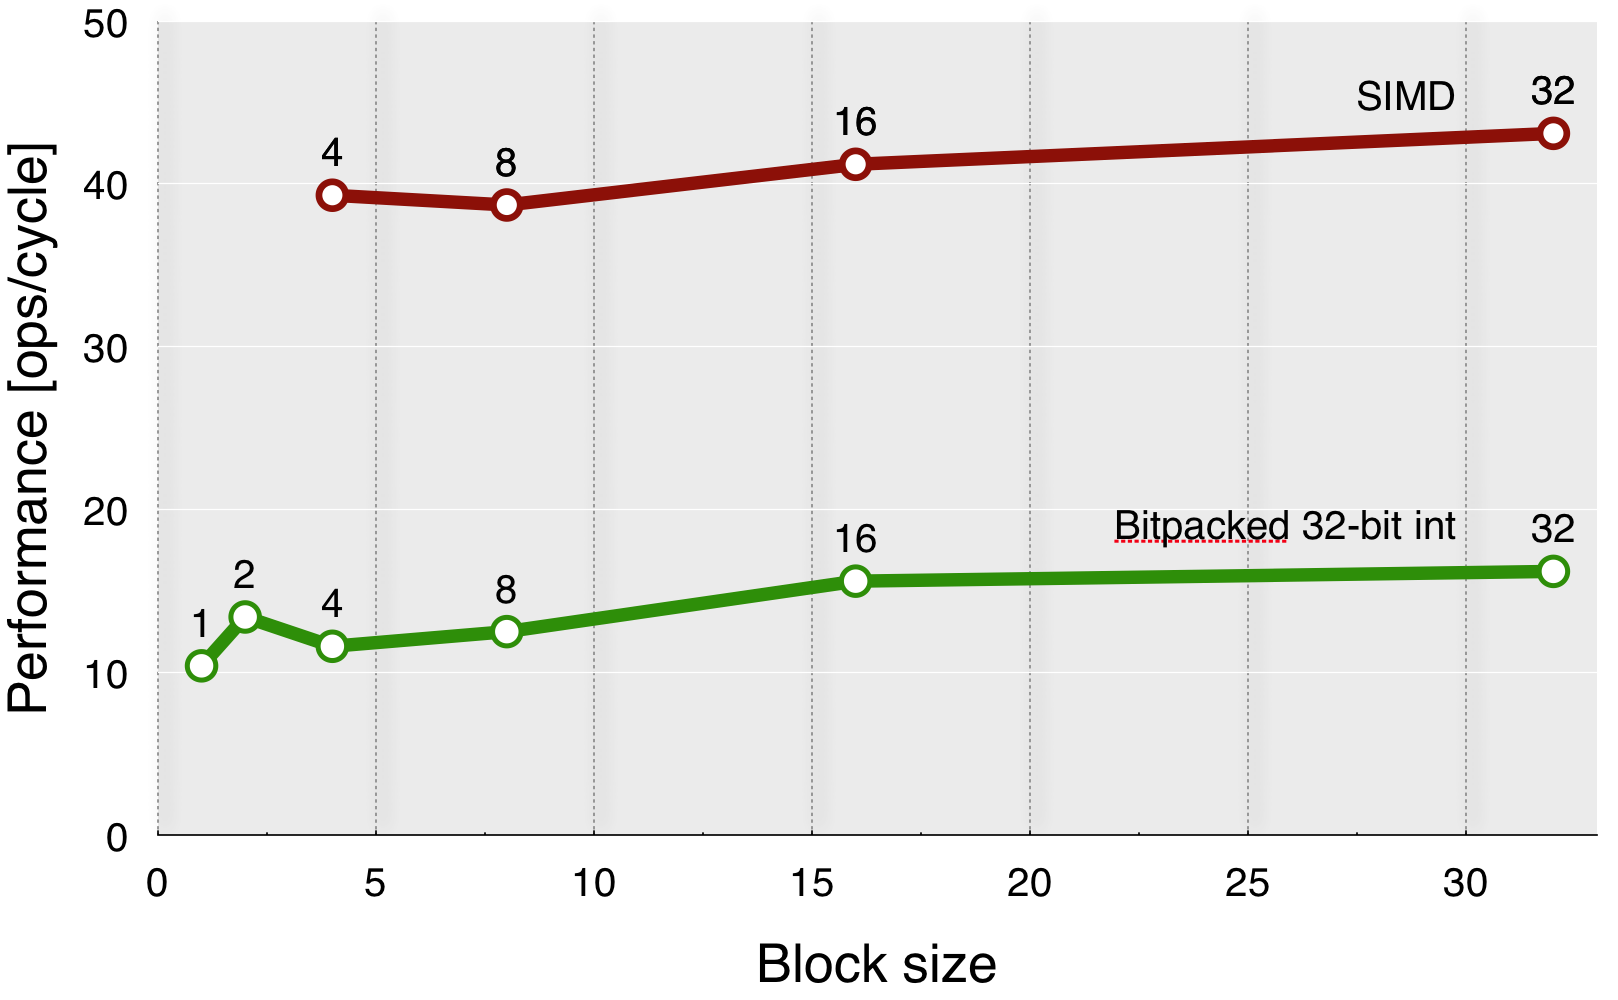
\includegraphics[width=0.85\textwidth]{graphs/UALL.png}
  \label{fig:benchmarking-uall}
  \caption{Comparison of bit-packed 32bit integer to bitpacked 128bit SIMD vector for different block sizes of the register blocking}
\end{figure*}

\begin{figure*}
  \centering
  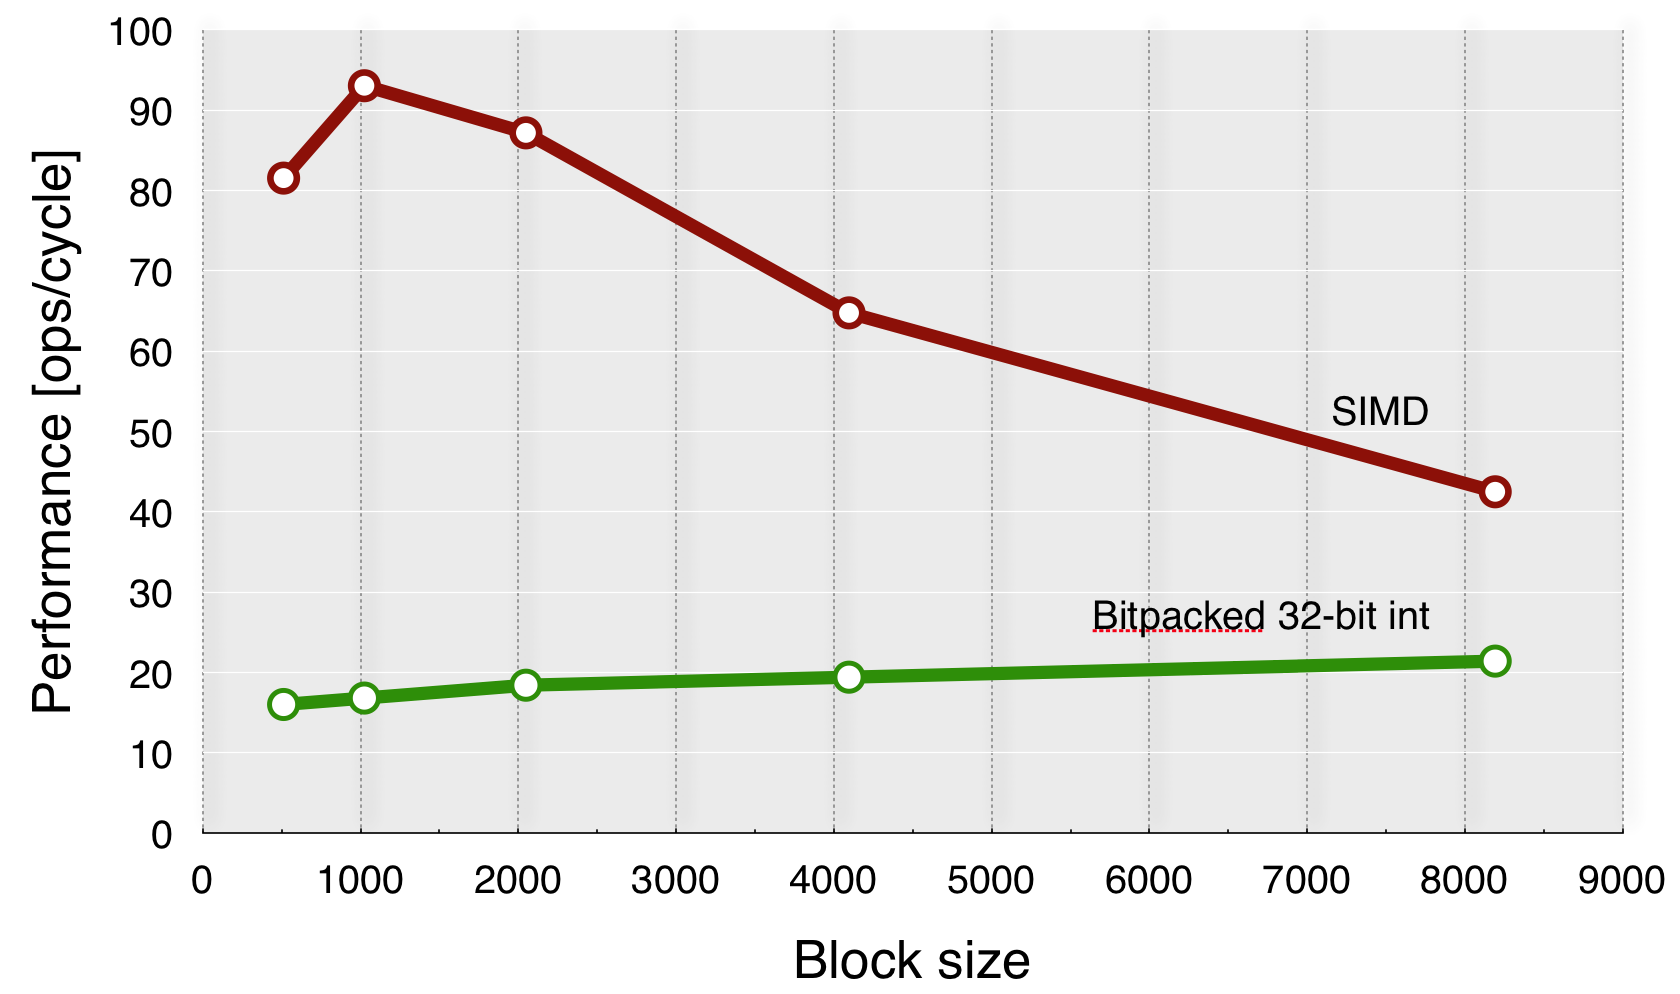
\includegraphics[width=0.85\textwidth]{graphs/Cache_size.png}
  \label{fig:benchmarking-cache}
  \caption{Comparison of bit-packed 32bit integer to bitpacked 128bit SIMD vector for different cache block sizes}
\end{figure*}

\begin{figure*}
  \centering
  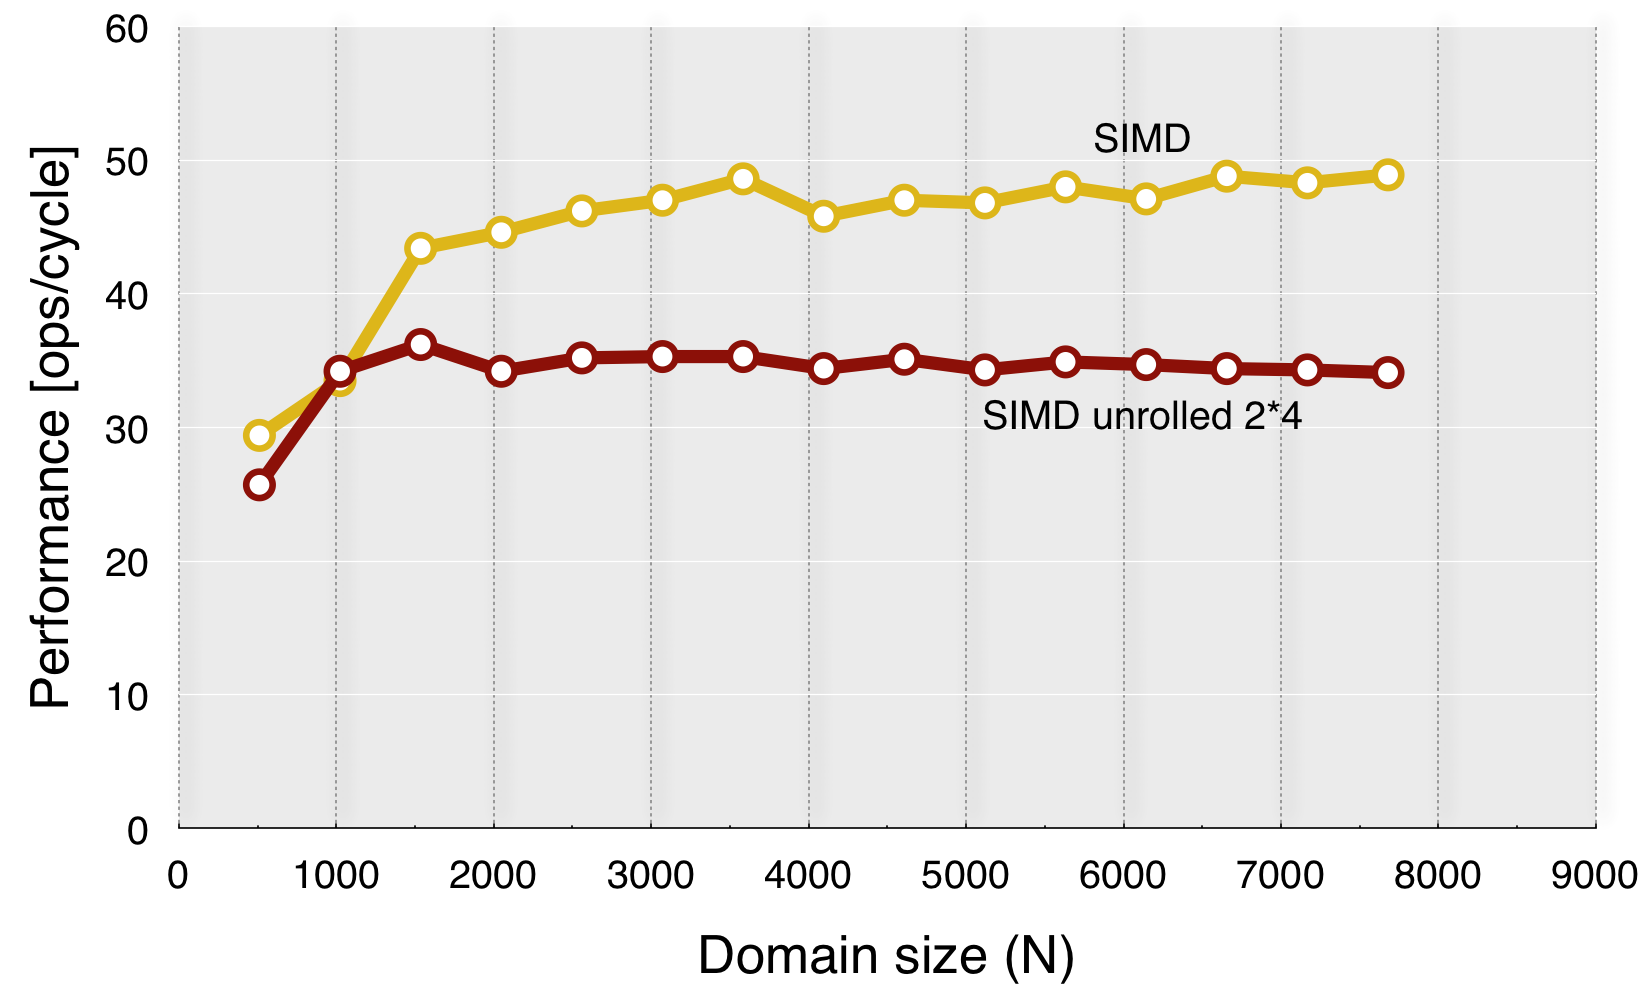
\includegraphics[width=0.85\textwidth]{graphs/Unrolling.png}
  \label{fig:benchmarking-unrolling}
  \caption{Comparison of 128-bit SIMD for different unroll factors. Note: The yellow non-unrolled version is partly unrolled by GCC}
\end{figure*}


Our algorithm was implemented using C++ and we have benchmarked it to see the difference between the algorithm as described in the paper and our different implementations.

Figure (1) shows our final results. We can see the difference from STL Map (as described in the paper) to our fastest solution is about 10 000x. The highest improvement is by going to dense matrices, but there is still a solid 100x to the final SIMD implementation.

Figure (2) shows performance for different block sizes of the register blocking. We have 16 SIMD registers available and it should thus be logical if we saw a bump or similar in that range. The GCC compiler does however make very clever optimizations which we did not get rid of which makes the result better and better with larger register loops due to more freedom given to the compiler in reordering and allocating registers.

Figure (3) shows the effect of different tiling sizes for the cache. We clearly see 1024 is the sweet spot here, and that it does not matter that much for the 32-bit bitpacked int version.

Figure (4) shows the effect unrolling of the register loops has on performance. We have experimented a bit and the one showed is the best one we could achieve. We are still ~25\% below the GCC compiler, which also does unrolling and is a lot better than us on this.

%Here you evaluate your work using experiments. You start again with a
%very short summary of the section. The typical structure follows.
%
%\mypar{Experimental setup} Specify the platform (processor, frequency, cache sizes)
%as well as the compiler, version, and flags used. I strongly recommend that you play with optimization flags and consider also icc for additional potential speedup.
%
%Then explain what input you used and what range of sizes. The idea is to give enough information so the experiments are reproducible by somebody else on his or her code.
%
%\mypar{Results}
%Next divide the experiments into classes, one paragraph for each. In the simplest case you have one plot that has the size on the x-axis and the performance on the y-axis. The plot will contain several lines, one for each relevant code version. Discuss the plot and extract the overall performance gain from baseline to best code. Also state the percentage of peak performance for the best code. Note that the peak may change depending on the situation. For example, if you only do additions it would be 12 Gflop/s
%on one core with 3 Ghz and SSE and single precision floating point.
%
%Do not put two performance lines into the same plot if the operations count changed significantly (that's apples and oranges). In that case first perform the optimizations that reduce op count and report the runtime gain in a plot. Then continue to optimize the best version and show performance plots.
%
%{\bf You should}
%\begin{itemize}
%\item Follow the guide to benchmarking presented in class, in particular
%\item very readable, attractive plots (do 1 column, not 2 column plots
%for this class), proper readable font size. An example is below (of course you can have a different style),
%\item every plot answers a question, which you pose and extract the
%answer from the plot in its discussion
%\end{itemize}
%Every plot should be discussed (what does it show, which statements do
%you extract).

\section{Conclusion}
Abstract interpretation in conjuction with Pentagon domain has proven itself as an efficient tool for
capturing many common programming errors. But in order to be practical, the most costly operations in the domain
have to be scalable. In this paper we used various techniques for optimizing the ``join'' operation. As a result the optimized
implementation is within 35\% of the theoretical maximum on our test hardware and is over 150x faster than 
the straighforward na\"ive approach (DM implementation). Some of the optimizations are also applicable in other areas in which
fast transitive closure is needed.

%Here you need to briefly summarize what you did and why this is
%important. {\em Do not take the abstract} and put it in the past
%tense. Remember, now the reader has (hopefully) read the paper, so it
%is a very different situation from the abstract. Try to highlight
%important results and say the things you really want to get across
%(e.g., the results show that we are within 2x of the optimal performance ... 
%Even though we only considered the DFT, our optimization
%techniques should be also applicable ....) You can also formulate next
%steps if you want. Be brief.

%\section{Further comments}
%
%Here we provide some further tips.
%
%\mypar{Further general guidelines}
%
%\begin{itemize}
%\item For short papers, to save space, I use paragraph titles instead of
%subsections, as shown in the introduction.
%
%\item It is generally a good idea to break sections into such smaller
%units for readability and since it helps you to (visually) structure the story.
%
%\item The above section titles should be adapted to more precisely
%reflect what you do.
%
%\item Each section should be started with a very
%short summary of what the reader can expect in this section. Nothing
%more awkward as when the story starts and one does not know what the
%direction is or the goal.
%
%\item Make sure you define every acronym you use, no matter how
%convinced you are the reader knows it.
%
%\item Always spell-check before you submit (to me in this case).
%
%\item Be picky. When writing a paper you should always strive for very
%high quality. Many people may read it and the quality makes a big difference.
%In this class, the quality is part of the grade.
%
%\item Books helping you to write better: \cite{Higham:98} and \cite{Strunk:00}.
%
%\item Conversion to pdf (latex users only): 
%
%dvips -o conference.ps -t letter -Ppdf -G0 conference.dvi
%
%and then
%
%ps2pdf conference.ps
%\end{itemize}
%
%\mypar{Graphics} For plots that are not images {\em never} generate (even as intermediate step)
%jpeg, gif, bmp, tif. Use eps, which means encapsulate postscript, os pdf. This way it is
%scalable since it is a vector graphic description of your graph. E.g.,
%from Matlab, you can export to eps or pdf.
%
%Here is an example of how to get a plot into latex
%(Fig.~\ref{fftperf}). Note that the text should not be any smaller than shown.
%
%\begin{figure}\centering
%  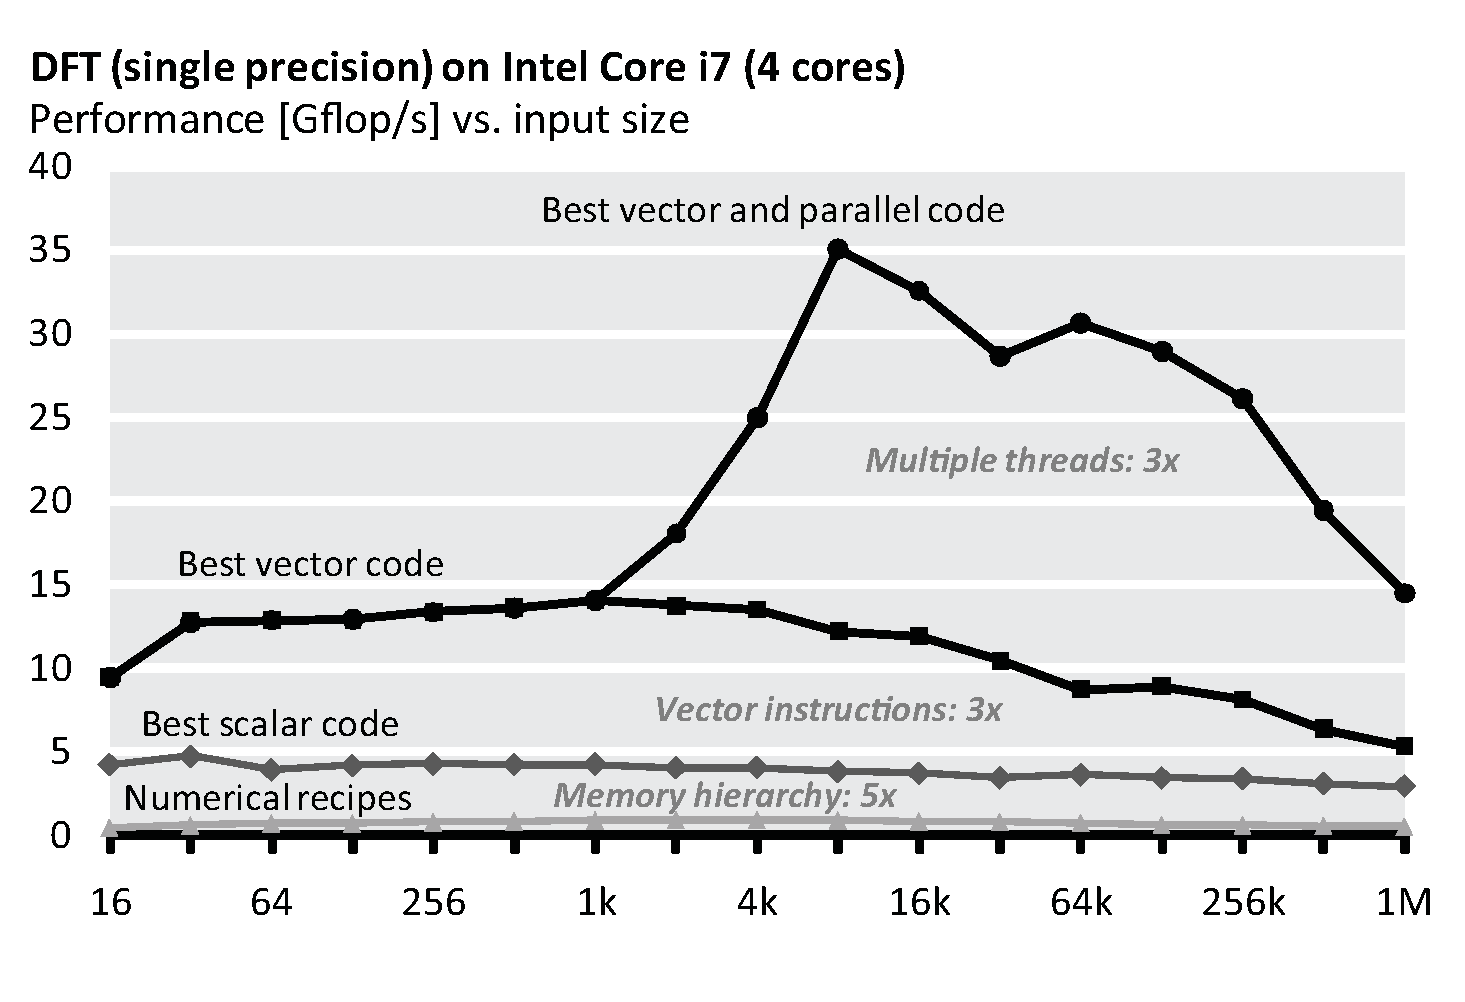
\includegraphics[scale=0.33]{dft-performance.eps}
%  \caption{Performance of four single precision implementations of the
%  discrete Fourier transform. The operations count is roughly the
%  same. {\em The labels in this plot are too small.}\label{fftperf}}
%\end{figure}
%



% References should be produced using the bibtex program from suitable
% BiBTeX files (here: bibl_conf). The IEEEbib.bst bibliography
% style file from IEEE produces unsorted bibliography list.
% -------------------------------------------------------------------------
\bibliographystyle{IEEEbib}
\bibliography{bibl_conf}

\end{document}

